\chapter{What is algebra?}

Algebra is the study of equations, for the most part equations involving variables.
That is because applications have unknowns and if 
the shape of the equation can tell us anything about the 
options to solve it, we shall want to take advantage of this.
Witness how we solve $ax^2+bx+c=0$ in one strategy despite it covering 
an infinite number of equations. Basic though it may seem that solution illustrates
the general arc of an algebra investigation.
\begin{center}
    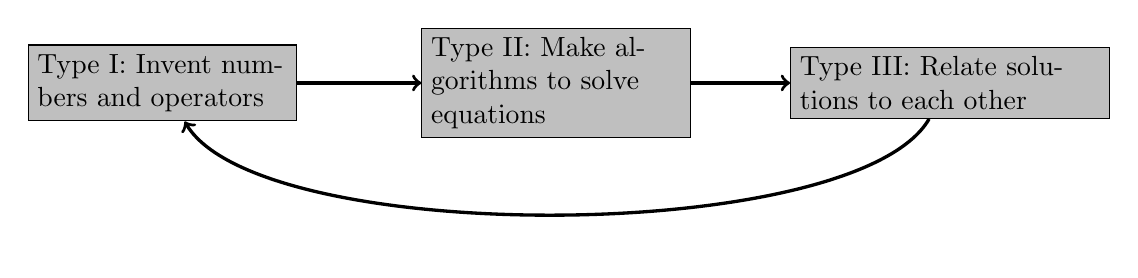
\begin{tikzpicture}
        \node[text width=1.25in, draw,fill=black!25] (a) at (0,0) {Type I: Invent numbers and operators};
        \node[text width=1.25in, draw,fill=black!25] (b) at (5,0) {Type II: Make algorithms to solve equations};
        \node[text width=1.5in, draw,fill=black!25] (c) at (10,0) {Type III: Relate solutions to each other};
        % \draw[very thick,->] (-4,0) -- (a);
        \draw[very thick,->] (a) -- (b);
        \draw[very thick,->] (b) -- (c);
        \draw[very thick,->] (c) edge[looseness=0.5,out=-120,in=-60] (a);
    \end{tikzpicture}
\end{center}
    
% \begin{enumerate}
%     \item What numbers lead to solutions existing? Do we need to invent $\sqrt{2}$
%     $i$, and possibly others?
%     \item If solutions exists, what algorithms find them? Complete the square, 
%         use a stock quadratic formula? Gaussian eliminate?
%     \item When multiple solutions, relate them to one another to simplify the answer.  
%     E.g.\ $\pm \sqrt{2}$, shift answers to a null space, use a basis.  Go 
%     back to 1 with these relations.
% \end{enumerate}
Childhood is mostly type I algebra.  Children learn to count and give these counts 
the usual names
\begin{center}
    % $0\defeq$ \underline{\hspace{5mm}}, 
    $1\defeq$ \StrokeOne,
    $2\defeq$ \StrokeTwo,
    $3\defeq$ \StrokeThree,
    $4\defeq$ \StrokeFour,
    $5\defeq$ \StrokeFive,...
\end{center}
Nothing gets the name $0$ (one theory is that the symbol reflects 
a dent in the sand left by removing a pebble to have none.)
Mathematicians and programmers see these \emph{natural numbers}
as produced by two rules, start with nothing, $0$, or take a successor 
$S(k)$ to natural number $k$ already created.  In notation we separate the 
cases by $|$ (read as ``or'') and define $\mathbb{N}$ by this pattern
\begin{align*}
    \mathbb{N} \defeq 0 \mid S(k)
\end{align*}

This creation of numbers inspires many others.
Imagine a string of characters in an alphabet \lstinline{Char:=['a','b',...,'z']}.
We start with either nothing (an empty string) or we add a character 
to a string we already have.  There is a little more going on here, we 
could add a character before or after the string we have.
\begin{lstlisting}[language=Hidris]
data String = Empty 
            | Prepend( head:Char, tail:String) 
            | Append( head:String, tail:Char)
\end{lstlisting}
Writing \lstinline{head:Char} or \lstinline{tail:String} 
indicates that head must come from the alphabet we chose 
and tail must be some already produced string, possibly empty.
Some readers might relate to a different dialect of 
programming such as the following
\begin{lstlisting}[language=Sava]
class String
  case Empty extends String
  case Prepend( head:Char, tail:String) extends String
sealed // No further cases
\end{lstlisting}
The head here caries around what we put in the list and the tail 
is what comes next in the list.  Observe the similarities:
\begin{align}
     2 & \defeq S(S(0)) \tag{$\mathbb{N}$}\\
 \text{\lstinline{"me"}} & \defeq \text{\lstinline{Prepend('m',Prepend('e',Empty))}}
\tag{String}
\end{align}
The left-hand sides are merely notation for what the data really is on the right.
Both the successor and the \lstinline{Prepend} are operators that generate 
new values.  So part of algebra is to generate new data; so, it is no wonder 
that it closely connections to computation.

\subsection*{Exercise}
\begin{enumerate}
    \item Mimic the String data type to make a list of integers (that is 
    switch from the alphabet to integers).

    \index{generics}
    \item Mimic the String data type to make a list of fixed by 
    unknown data of type $A$, call it \lstinline{List[A]}.\footnote{
    Alternatives include \lstinline{List a} and \lstinline{List<A>}. 
    Search for \emph{generics} in your programming language to learn more.
    }

\end{enumerate}
\index{nil}\index{cons}\index{list}
Historically \lstinline{Empty} for lists is called \lstinline{Nil} 
and \lstinline{Prepend} is called \lstinline{Cons}.


Children also learn to add, whatever that means conceptually, it obeys 
another simple pattern.
\begin{align*}
    m+n & \defeq\left\{ 
    \begin{array}{ll}
        n & m = 0\\
        S(n+k) & m=S(k)
    \end{array}
    \right.
\end{align*}
So does $2+4=6$?  We can test this out.
\begin{align*}
    \text{\StrokeTwo}+\text{\StrokeFour} & = \text{\StrokeOne}~ \big(\text{\StrokeOne} +\text{\StrokeFour}\big)\\
    & = \text{\StrokeOne}~ \big( \text{\StrokeOne}~\big(\underline{\hspace{5mm}}+\StrokeFour\big)\big)\\
    & = \text{\StrokeOne}~ \big( \text{\StrokeOne}~\StrokeFour\big)\\
    & = \text{\StrokeOne}~ \text{\StrokeFive}.
\end{align*}


A natural number is either $0$, or a successor 
$S(k)$ to 
another natural number $k$.  Often this is expressed as a 
definition where $\mid$ stands for separating cases, 
for example:
\begin{align*}
    \mathbb{N} \defeq 0 \mid S(k)
\end{align*}
So $0$ is ``zero'', and $1$ is just a symbol representing $S(0)$, 
$2\defeq S(S(0))$ and so on.  Replace $S$'s with tally marks (not to be 
confused with `$|$' used as an ``or'' above)
we recover childhood counting:
\begin{center}
    $0\defeq$ \underline{\hspace{5mm}}, 
    $1\defeq$ \StrokeOne,
    $2\defeq$ \StrokeTwo,
    $3\defeq$ \StrokeThree,
    $4\defeq$ \StrokeFour,
    $5\defeq$ \StrokeFive,...
\end{center}
The point is, the successors are not so much a function 
moving around the numbers we have, it actually is a producer 
of numbers. 

, find distances of
length $\sqrt{2}$, learn about imaginary numbers and $\pi$.  The shift to $\pi$
signals the shift to type II because $\pi$ is such a fiddly number that it
makes sense to leave it alone moving it round solely by rules of algebra until
the end when we might replace with with 3.14 or a better approximation. For
practical purposes $\pi$ is the first quantity used as a variable. 

High school algebra is nearly all type II, and mostly following al
Khwarizmi's \emph{al Jabr}---the method of balancing parts, which today is
called Algebra.  Move over Euclid, al Khwarizmi's method made people money,
settled land disputes, calculated grain totals and arguably did more to make
math a necessity for average people than any other source. His name has passed
down to modern life as the word \emph{algorithm}. At this stage students are
told  that polynomials of degree $d$ have $d$ complex roots.  Perhaps because
some non-algebraist call this fact ``the fundamental theorem of algebra'' (it's
not) this seems a good place to leave algebra for calculus or leave math for
good.  Most people never reach a type 3 problem.

You are one of the few who have heard of type 3 algebra.
You have seen the solving linear equations gives you back often infinitely many 
answers and you don't have time nor the interest to write down infinitely many answers.
You know that this can be done with a basis.  The next example is even more 
greedy.  Why write down $d$ roots to a $d$ degree polynomial?!  Instead, you 
want to write down one solution and sprinkle in some pattern to explain how you 
might find all the others.  Think back to 
$x=\frac{-b\pm \sqrt{b^2-4ac}}{2a}$ solving $ax^2+bx+c=0$ (with $a\neq 0$).
That `$\pm$' trick saved you thinking of two roots.  Ever solved $x^6-1=0$ by 
using $x=e^{(2\pi i/6) t}$ thinking of rotating around by 60 degrees?  
These relationships turned out to have a name (groups) and were the first type 3 
algebra.

This is where the heavy weights got
involved: Lagrange made a formula for quartic polynomials from a primitive
concept of groups but he got distracted by a fluke concerning symmetric polynomials 
and missed out on the eventual full solution by Galois.
Gauss showed that construction by ruler and compass produces only numbers 
that are iterated applications of square-roots by observing what in today's 
language would say that the group of relations is nilpotent. 
Abel found a specific obstacle with $x^5-x+1=0$ by showing that if its relations 
were to be solvable they would create contradictions with facts from calculus,
the first proof that not all polynomials are solvable by radicals.  
Galois characterizes all such polynomials by describing what their type 3
algebra would look like.  Both men died tragically and without their work being 
understood until after their young deaths.

Here I should settle a confusion in the subject.  Abel and Galois did 
not show that the quintic has no solutions!  That would fly in the 
face of  Gauss' ``fundamental theorem 
of algebra'' (a 5th degree polynomial has 5 complex roots).  
What Abel and Galois proved is that roots of these polynomials where not 
of the form hinted at by the solutions for 1,2,3 and 4th degree polynomials.
Take for example al Khwarizmi's quadratic formula gives roots of the form 
$\frac{-b}{2a}\pm \frac{1}{2a}\sqrt{b^2-4ac}$, where $a,b,c$ are numbers we 
already created.  Cardano's cubic formula goes a step further.  Given 
numbers $a,\ldots, g$ already created, then solutions to the cubic can 
be made in the following form.
\[
    a+b\sqrt{c}+d\sqrt[3]{e+f\sqrt{g}}.
\]
Lagrange's quartic formula gives solutions now involving rational 
linear combinations of fourth roots.  When a number is a linear combination 
of $n$-th roots of iteratively created numbers then we say that number 
is \emph{radical}.  That the quintic is not solvable by radicals just means 
that to factor quintics and higher students need to go back to a type 1 problem:
invent new constructions of numbers. In fact, history had already done this 
for degrees 2,3.  For example, if $b^2-4ac<0$ then the solutions may be written as
\begin{align*}
    x & = \sqrt{\frac{c}{a}}\cos\theta \pm \sqrt{\frac{c}{a}}\sin\theta
    & 
    \theta & = \cos^{-1}\frac{-b}{2\sqrt{ac}}
\end{align*}
The cubic equations can likewise be solved with trigonometry.  So Abel and Galois 
point the way to revisiting how we build numbers and finding new methods.  That is,
the outcome of type 3 algebra was a need to build new type 1 algebra.

This feedback look has been hard at work for more than a century.  These new
type 1 problems lead to rings and modules.  That lead to algorithms and
representation theory to solve type 2 problems with those numbers.  Those
solutions generated new relations, more groups (type 3), but also new type 1
algebras (Clifford, Lie, Hecke, and Hopf to name a few). The iteration continues. 

As a final remark, we should settle one last potential confusion.
The fundamental theorem of algebra already told us the shape of roots,
i.e.\ complex numbers.  Why not stop here?  Answer this yourself: 
what are the roots of  $x^2=2$?  If you thought $x=\pm\sqrt{2}$ and not $x\approx \pm 1.41$ then you 
appreciate the difference.  By prescribing $x=\pm \sqrt{2}$ we both solve nothing 
(its just notation) and everything (this solution truly works).  This gets a 
a philosophical position that numbers are made up to mean what they can do. 
Real numbers are made up to mean that finite patterns that stay close together 
(Cauchy sequences) can in fact be considered as numbers (they converge to themselves,
which means nothing but lets there be real numbers).

Radical numbers like $\sqrt{2}$ are another form of invention, a number that when 
squared is $2$.  It is freeing to think this way because we can make such numbers 
precisely with ease.  For example $\begin{bmatrix} 0 & 2\\ 1 & 0\end{bmatrix}$
squares to $\begin{bmatrix} 2 & 0 \\ 0 & 2 \end{bmatrix}$ which gives precise 
calculations.  But for some situations precision wont be important and we can 
use the approximation $1.41^2\approx 2$.  Algebra therefore sees the matrix and the decimal 
examples of $\sqrt{2}$ as interchangeable. 
To algebra, $\sqrt{2}$ is a property, not so much a number.  Because of this 
we can imagine many more creative algorithms to work with these numbers.

For the purposes of solving it is important to have both 
but exact and approximate solutions.
To expose this difference 
look no further than finding the eigenvalues of a matrix.
\begin{align*}
    \begin{bmatrix}
        -9 & 7 & -12 & 6\\
        -3 & 5 & -4 & 6\\
        7 & -5 & 8 & -2\\
        2 & -2 & 4 & -4
    \end{bmatrix}
\end{align*}
With 64 bit floating points in Julia, my computer printed out 
\begin{lstlisting}
    julia> eigvals([-9 7 -12 6; -3 5 -4 6; 7 -5 8 -2; 2 -2 4 -4])
    4-element Vector{ComplexF64}:
     -0.0005295477729425071 - 0.0005295190134323146im
     -0.0005295477729425071 + 0.0005295190134323146im
      0.0005295477729438736 - 0.0005295765047025466im
      0.0005295477729438736 + 0.0005295765047025466im   
\end{lstlisting}
But actually this matrix has a single eigenvector $0$ and is not diagonalizable 
but instead it is conjugate to a nilpotent matrix:
\begin{align*}
    \begin{bmatrix}
        -9 & 7 & -12 & 6\\
        -3 & 5 & -4 & 6\\
        7 & -5 & 8 & -2\\
        2 & -2 & 4 & -4
    \end{bmatrix}
    & =
    \begin{bmatrix}
        1 & 2 &  1 & 2\\
       -1 & 2 & -1 & 2\\
         0 & 1 &  1 & 0\\
         1 & 0 &  1 &  1
   \end{bmatrix}^{-1}
   \begin{bmatrix}
        0 & 4 & 0 & 0\\
        0 & 0 & 4 & 0\\
        0 & 0 & 0 & 4\\
        0 & 0 & 0 & 0
    \end{bmatrix}
    \begin{bmatrix}
         1 & 2 &  1 & 2\\
        -1 & 2 & -1 & 2\\
          0 & 1 &  1 & 0\\
          1 & 0 &  1 &  1
    \end{bmatrix}
\end{align*}
Solutions to equations are not stable under approximations.




\section{Everything is variable}
You probably already know every color, shape, and pattern of 
equation you will ever need.  Compare these two equations
\begin{align*}
    x^2+y^2 & \equiv 0 \pmod{541} 
    & 
    \frac{\partial^2 f}{\partial x^2}+\frac{\partial^2 f}{\partial y^2} & =0.
\end{align*}
Can you stop yourself from seeing them as related?
These equations concern entirely different things.  On the left $0$ can 
equal 541.  On the right $0$ is functions on the $xy$-plane.
Yet, the similarities as equations shine through.  Why? Is it because $0$, 
$+$, and  powers of $2$ are general concepts, ``abstractions''.  This doesn't connect them to
polarizing art movements nor render the concept inapplicable.  Abstract here,
and everywhere, means to study by limited attributes.  That's how we do all
math and science.  So when we abstract the equation on the left we forget
about mod 541 and the precise meaning of these numbers.  On the right we forget
about functions and the notions of derivatives.  We are left with just $0$, 
$+$, and squares and where they sit.  We abstract both to a common equation
\[
    x^2+y^2=0.
\]
In fact, even the equality was an abstraction which could vary from context to context.
With such flexibility a small number of symbols and their grammar are enough to capture 
the huge variety of equations we encounter in real life.

\begin{quote}
    \textbf{The power of algebra is that every symbol 
    in an equation is a variable, especially the equals sign.}
\end{quote}

\section{Inventing numbers}
Now since every symbol in an equation is a variable we have new powers 
to solve equations.  Look to the humble 
\[
    x^2+1=0.
\]
By our own view, right now this is nothing but variables, so it means nothing to
solve this.  But, drop this into a context such as decimal numbers $\mathbb{R}$
and the understanding is to replace $1\defeq 1.0$, $0\defeq 0.0$, $+$ is
substituted for addition of decimals, and square is by multiplying decimals.
Equality now means two equal decimals, or in practice two decimal numbers that are close enough 
to be considered equal.  The only remaining unknown is $x$, but as everyone 
knows, $0\leq x$ or $x<0$ so in both cases $-1<0\leq x^2$.

The power of variable everything is that we are not stuck with the real numbers.
Let us replace everything with complex numbers $\mathbb{C}$. Substitute $0\defeq
0+0i$, $1=1+0i$, $(a+bi)+(c+di)\defeq (a+b)+(c+d)i$, and
$(a+bi)^2=(a^2-b^2)+2abi$.  Now we find $\pm i$ are the solutions. Solutions do
exist!  Since they exist we can return to a problem and ask if the solutions we 
found will do the job.  Maybe not, or maybe we should revisit our models and 
see these solutions as predicting the presence of previously unknown realities.

Why stop here? Quaternions have $\hat{\i}^2=\hat{\j}^2=\hat{k}^2=-1$;
so, at least 6 solutions to $x^2+1=0$.  Even more.  Try $(2\times 2)$-matrices, I
bet you can find infinitely many matrices $M$ where $M^2=-I_2$.  This is the method
of algebra: dream up new numbers that might be used to solve equations.  Alter
their properties, e.g.\ drop the order of real numbers and you can get complex
solutions.  Drop commutative multiplication of complex numbers and you might get
infinite solutions.  Learn enough by this process and we can begin to predict if
solutions are to be expected and fathom algorithms to find them when they do
exist. When the solutions become infinite we find ways to parameterize them with
smaller data such as a basis.

Don't forget equality is variable too!  Suppose we wanted to solve $x^{541}+x+1=0$
using only integers.  Replace equality 
with $\equiv$ modulo 2 and ask for a whole number $x$ that solves
\begin{align*}
    x^{541}+x+1\equiv 0\pmod{2}.
\end{align*}
All integers in this equality become either $0$ or $1$, but neither will solve 
this equation.  By varying equality we confirm there are no solutions.

This is why so much of algebra today is concerned with making new numbers and 
searching out which equalities (congruences) can be used on new numbers.  It is 
the front line of algebra, the first question that must be concurred.  And it part 
of why so much research on algebra doesn't even feature solving equations because 
the goal is to have numbers ready for whatever equations show up.

\begin{quote}
    \textbf{The first method of algebra is to invent numbers: their constants, their 
    operations, their rules.  We call these ``algebras''.}
\end{quote}

\section{Computation}
Algebra is the computational wing of mathematics.  

Look to calculus.
We obviously work with limits and derivatives to recover Rolle's theorem 
and the significance of $f'(x)=0$.  But when we want to find such $x$ we
inevitably are left to solve equations, like $x^2-x-3=0$, which we do by algebra.  

Switch to topology.   Roll up a stretchy sheet of plastic along the following 
Van Kampen patterns  viewed in Figure~\ref{fig:vanKampen} to make a torus $\mathbb{T}^2$ 
and a Klein bottle $\mathbb{K}$.  These are different, right?  Why?  Of course we use topology 
to prove the interesting bit, like the Seifert-van Kampen theorem: the loops 
$\pi_1(M^2)$ on a surfaces $M^2$ can each be described as a sequence of blue loops $b$ and red loops $r$.
Loops that contract to nothing can be read along the boundary.  Hence,
\begin{align*}
    \pi_1(\mathbb{T}^2) &= \text{ words over }\{b,r\} \text{ rewritten by }br=rb;
    \\
    \pi_1(\mathbb{K}^2) &= \text{ words over }\{b,r\} \text{ rewritten by } r=brb. 
\end{align*}
We use algebra to compute that those numbers are not the same so neither are the two spaces.
\begin{figure}[!htbp]
    \centering
\begin{tikzpicture}
    \node (T) at (-3,0) {\begin{tikzpicture}
        \fill[color=black!25] (0,0) rectangle (2,2);
        \draw[thick,->, red] (0,0) -- ++(2,0);
        \draw[thick,->,red] (0,2) -- ++(2,0);
        \draw[thick,->>, blue] (0,0) -- ++(0,2);
        \draw[thick,->>,blue] (2,0) -- ++(0,2);
    \end{tikzpicture}};
    \node (K) at (3,0) {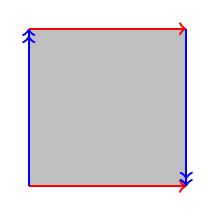
\begin{tikzpicture}
        \fill[color=black!25] (0,0) rectangle (2,2);
        \draw[thick,->, red] (0,0) -- ++(2,0);
        \draw[thick,->,red] (0,2) -- ++(2,0);
        \draw[thick,->>, blue] (0,0) -- ++(0,2);
        \draw[thick,->>,blue] (2,2) -- ++(0,-2);
    \end{tikzpicture}};

    \node (Tv) at (-3,-3) {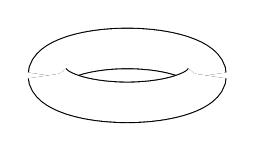
\begin{tikzpicture}[yscale=cos(70)]
        \draw[double distance=5mm] (0:1) arc (0:180:1);
        \draw[double distance=5mm] (180:1) arc (180:360:1);
      \end{tikzpicture}};
    \node (Kv) at (3,-3) {\begin{tikzpicture}[scale=0.25,use Hobby shortcut]
        \draw ([closed,blank=soft]0,0)
        \foreach \pt in {
        (-2,2),
        (2,2),
        (2,-2),
        (-2,-2),
        ([blank]-2,-1),
        (-1,-1),
        (1,-2),
        ([blank=soft]1,2),
        ([blank=soft]-1,1),
        (-3,3),
        (6,4.5),
        (4.5,-4.5),
        (-2.5,-6)
        } {
        .. ++\pt
        };
        % \draw[dashed,use previous hobby path={invert soft blanks}];
        \draw (0,0) .. +(-1,-1) .. ++(-2,-1);
        \draw[dashed] (0,0) .. +(-1,-.75) .. ++(-2,-1);
        \draw (-2.45,-3.9) .. +(3.3,-.75) .. (4.2,-3.95);
        \draw[dashed] (-2.45,-3.9) .. +(4.3,.5) .. (4.2,-3.95);
        \end{tikzpicture}};

        \draw[thick,->] (T) -- (Tv);
        \draw[thick,->] (K) -- (Kv);
    \end{tikzpicture}
    \caption{A torus and Klein bottle, with thanks to 
    \url{https://tex.stackexchange.com/q/77606/86}.}\label{fig:vanKampen}
\end{figure}

Other fields?  How many times in applied math, number theory, or combinatorics
do we end up solving something even if just a linear equation, in order to get 
a final answer?  You don't have to be convinced but the evidence is there.

Yet most of us do not want to be computers.  So what does an algebraist do 
when the questions come down to computing?  We put our energy into crafting 
algorithms to solve these problems.  In fact the word ``algorithm'' comes 
from al Khwarizmi whose influential book \emph{al Jabr} (the method of parts)
gave use the first detailed explanations of algebra.  Half of that book 
is a list of story problems solved by various algorithms in algebra.
If you are concerned that this now trends to computer science, well know that 
computer science cares more about the data structures than about any algorithms.
Just like counting get faster with an abacus, algebraic algorithms get better 
with data structures.  So these two worlds interact but care deeply about 
different parts of the problem.